\documentclass[
  11pt,
  letterpaper,
   addpoints,
   answers
  ]{exam}

\usepackage{../exercise-preamble}
\usepackage{float}
\usepackage{tikz}
\usepackage{cancel} % Para mostrar la sustitución sin(theta) -> theta
\usetikzlibrary{decorations.pathmorphing}

\begin{document}
\pagestyle{headandfoot}
\firstpagefooter{ }{Página \thepage\ de \numpages}{ }
\runningfooter{ }{Página \thepage\ de \numpages}{ }

\noindent
\begin{minipage}{0.47\textwidth}
\includegraphics[width=\textwidth]{../fcfm_die.png}
\end{minipage}
\begin{minipage}{0.53\textwidth}
\begin{center} 
\large\textbf{Introducción a la Física Moderna} (F1100-5) \\
\large\textbf{Clase auxiliar 7} \\
\normalsize Prof.~ Rodrigo Soto.\\
\normalsize Prof.~Aux.~Erik Sáez - Javiera Toro 
\end{center}
\end{minipage}
\vspace{0.5cm}
\noindent
\vspace{.85cm}

\begin{questions}
%--------------------------
\question Un buque en reposo sobre aguas profundas está equipado con un sonar que envía pulsos de sonido de $20\,\mathrm{MHz}$. Los pulsos reflejados en la superficie de un submarino ubicado directamente debajo del barco se demoran $0{,}06\,\mathrm{s}$ en regresar al barco y tienen una frecuencia de $19{,}979\,\mathrm{MHz}$. Considere que la velocidad del sonido en el agua de mar es $1{,}48\,\mathrm{km/s}$.

\begin{figure}[H]
\centering
\begin{tikzpicture}[>=Latex,scale=1]
  % Agua (superficie y relleno)
  \fill[blue!10] (-5,0) rectangle (5,-5);
  \draw[blue!60,very thick] (-5,0)--(5,0);
  \node[blue!60,above right] at (-5,0) {Superficie del mar};

  % Barco (simple)
  \fill[gray!30] (-1.3,0) rectangle (1.3,0.6);
  \fill[gray!30] (-1.3,0.6)--(1.3,0.6)--(0,1.1)--cycle;
  \node[align=center] at (0,1.35) {Barco en reposo};
  % Transductor
  \coordinate (tx) at (0,0);
  \fill[red] (tx) circle (2pt);
  \node[above right] at (tx) {Transmisor SONAR};

  % Submarino (simple), directamente debajo
  \coordinate (refl) at (0,-3.0); % punto de reflexión (techo del submarino)
  \begin{scope}[shift={(0,-3.3)}]
    \draw[fill=gray!55] (-2.0,-0.3) .. controls (-1.2,0.5) and (1.2,0.5) .. (2.0,-0.3)
      -- (2.0,-0.7)--(-2.0,-0.7)--cycle;
    \draw[fill=gray!55] (-1.5,0.0) rectangle (-1.0,0.35); % vela
    \node[below] at (0,-0.7) {Submarino};
  \end{scope}

  % Pulsos de sonido (ida y vuelta)
  \draw[red,thick,->] (tx) -- (refl)
    node[midway,right,xshift=4pt] {$f_s=20~\text{MHz}$};
  \draw[red,thick,->] (refl) -- (tx)
    node[midway,left,xshift=-30pt] {$f_r=19.979~\text{MHz}$};

  % Profundidad (doble flecha) y tiempo de eco
  \draw[<->,thick] (-0.7,0) -- (-0.7,-3.0)
    node[midway,left] {$d$};
  \node[right] at (0.15,-2) {$\Delta t=0.06~\text{s}$ (ida y vuelta)};

  % Parámetros dados
  \node[align=left,anchor=west] at (-4.8,-4.4) {$v_{\text{sonido}}=1.48~\text{km/s}$};
  % Velocidad vertical del submarino (a determinar)
  \draw[->,thick] (1.7,-3.0) -- ++(0,-0.9);
  \node[right] at (2,-3.45) {$v_z~?$};
\end{tikzpicture}
\caption{Esquema (no a escala) del sonar: el barco emite un pulso hacia abajo que se refleja en la parte superior del submarino. Se mide el tiempo de eco $\Delta t$ y un corrimiento Doppler entre $f_s$ y $f_r$; con $v_{\text{sonido}}$ se obtiene la profundidad $d$ y a partir del corrimiento, la velocidad vertical $v_z$.}
\end{figure}

\begin{parts}
\part Encuentre la profundidad del submarino.
\part Encuentre la velocidad vertical del submarino.
\end{parts}
%--------------------------
\begin{solution}
\subsection*{Resolución 1.1 }

Para encontrar la profundidad del submarino, utilizamos la información del tiempo que tarda el pulso de sonar en regresar al barco.

\begin{itemize}
    \item Tiempo total de ida y vuelta: $t = 0{,}06\,\mathrm{s}$
    \item Velocidad del sonido en agua de mar: $v = 1{,}48\,\mathrm{km/s} = 1480\,\mathrm{m/s}$
\end{itemize}


El pulso de sonar debe viajar desde el barco hasta el submarino y luego regresar al barco. Por lo tanto, el pulso recorre una distancia total de $2d$, donde $d$ es la profundidad del submarino.

La relación entre distancia, velocidad y tiempo es:
\begin{equation}
\text{distancia total} = \text{velocidad} \times \text{tiempo total}
\end{equation}

Sustituyendo los valores conocidos:
\begin{align}
2d &= v \times t \\
2d &= 1480\,\mathrm{m/s} \times 0{,}06\,\mathrm{s} \\
2d &= 88{,}8\,\mathrm{m}
\end{align}

Despejando la profundidad $d$:
\begin{align}
d &= \frac{88{,}8\,\mathrm{m}}{2} \\
d &= 44{,}4\,\mathrm{m}
\end{align}

Por lo que finalmente la profundidad del submarino es $\boxed{44{,}4\,\mathrm{m}}$.

\subsection*{Resolución 1.2 }

Para encontrar la velocidad vertical del submarino, utilizamos el efecto Doppler observado en la frecuencia del pulso reflejado.

\begin{itemize}
    \item Frecuencia emitida: $f_0 = 20\,\mathrm{MHz} = 20 \times 10^6\,\mathrm{Hz}$
    \item Frecuencia recibida: $f = 19{,}979\,\mathrm{MHz} = 19{,}979 \times 10^6\,\mathrm{Hz}$
    \item Velocidad del sonido: $v = 1480\,\mathrm{m/s}$
\end{itemize}


En este caso tenemos un \textbf{doble efecto Doppler} porque la onda sonora realiza un viaje de ida y vuelta:
\begin{enumerate}
    \item \textbf{Primera etapa}: Del barco (fuente en reposo) al submarino (observador en movimiento)
    \item \textbf{Segunda etapa}: Del submarino (ahora actúa como fuente en movimiento) de vuelta al barco (observador en reposo)
\end{enumerate}

Para el doble efecto Doppler, debemos analizar cada etapa por separado usando la fórmula general del efecto Doppler:

\begin{equation}
f' = f_0 \left(\frac{v \pm v_r}{v \pm v_s}\right)
\end{equation}

donde $v_r$ es la velocidad del receptor y $v_s$ es la velocidad de la fuente (signos: $+$ si se acercan, $-$ si se alejan).

\textbf{Derivación paso a paso:}

\begin{enumerate}
    \item \textbf{Barco → Submarino}: 
    \begin{itemize}
        \item Fuente: barco (en reposo) $\rightarrow v_s = 0$
        \item Receptor: submarino (alejándose) $\rightarrow v_r = -v_{sub}$ (negativo porque se aleja)
    \end{itemize}
    \[f_1 = f_0 \left(\frac{v - v_{sub}}{v}\right)\]
    
    \item \textbf{Submarino → Barco}: 
    \begin{itemize}
        \item Fuente: submarino (alejándose) $\rightarrow v_s = -v_{sub}$ (negativo porque se aleja)
        \item Receptor: barco (en reposo) $\rightarrow v_r = 0$
    \end{itemize}
    \[f = f_1 \left(\frac{v}{v - (-v_{sub})}\right) = f_1 \left(\frac{v}{v + v_{sub}}\right)\]
\end{enumerate}

Combinando ambos efectos:
\begin{align}
f &= f_0 \left(\frac{v - v_{sub}}{v}\right) \left(\frac{v}{v + v_{sub}}\right) \\
f &= f_0 \left(\frac{v - v_{sub}}{v + v_{sub}}\right)
\end{align}

Como la frecuencia recibida ($19{,}979\,\mathrm{MHz}$) es \textit{menor} que la emitida ($20\,\mathrm{MHz}$), confirmamos que el submarino se aleja del barco.

Donde tenemos que:
\begin{itemize}
    \item $f$: Frecuencia final recibida por el barco
    \item $f_0$: Frecuencia original emitida por el barco
    \item $v$: Velocidad del sonido en el agua de mar
    \item $v_{sub}$: Velocidad del submarino (valor positivo, alejándose)
\end{itemize}

El signo de $v_s$ indica la dirección: positivo si el submarino se aleja del barco (frecuencia menor), negativo si se acerca (frecuencia mayor).

Despejando $v_s$:
\begin{align}
\frac{f}{f_0} &= \frac{v - v_s}{v + v_s} \\
\frac{f}{f_0}(v + v_s) &= v - v_s \\
\frac{f}{f_0} \cdot v + \frac{f}{f_0} \cdot v_s &= v - v_s \\
\frac{f}{f_0} \cdot v_s + v_s &= v - \frac{f}{f_0} \cdot v \\
v_s\left(\frac{f}{f_0} + 1\right) &= v\left(1 - \frac{f}{f_0}\right) \\
v_s &= v \cdot \frac{1 - \frac{f}{f_0}}{\frac{f}{f_0} + 1}
\end{align}

Calculando la relación de frecuencias:
\begin{align}
\frac{f}{f_0} &= \frac{19{,}979 \times 10^6}{20 \times 10^6} = \frac{19{,}979}{20} = 0{,}99895
\end{align}

Sustituyendo en la ecuación:
\begin{align}
v_s &= 1480 \cdot \frac{1 - 0{,}99895}{0{,}99895 + 1} \\
v_s &= 1480 \cdot \frac{0{,}00105}{1{,}99895} \\
v_s &= 1480 \cdot 0{,}000525 \\
v_s &= 0{,}777\,\mathrm{m/s}
\end{align}

Por lo que finalmente la velocidad vertical del submarino es $\boxed{0{,}78\,\mathrm{m/s}}$ alejándose del barco.

\end{solution}
%--------------------------
\question Se realiza un experimento de doble rendija usando un láser de He-Ne ($\lambda = 633\,\mathrm{nm}$). Luego, se coloca una placa muy delgada de vidrio ($n = 1{,}5$) sobre una de las ranuras. Se observa que el punto central en la pantalla está ahora ocupado por la que había sido la franja oscura correspondiente a $m = 10$. ¿Cuán grueso es el vidrio?

Considere que la pantalla está ubicada muy lejos, de manera que vale la aproximación paraxial (todos los ángulos son muy pequeños).
%--------------------------
\begin{solution}
\subsection*{Resolución 2.1}

En el experimento de doble rendija original, sin la placa de vidrio, el patrón de interferencia se debe a la diferencia de camino óptico entre la luz que pasa por cada rendija. Las franjas brillantes aparecen cuando la diferencia de camino es un múltiplo entero de la longitud de onda, y las franjas oscuras aparecen cuando la diferencia es un múltiplo impar de media longitud de onda.


La condición para una franja oscura en el experimento original es:
\begin{equation}
\Delta = d \sin \theta = \left(m + \frac{1}{2}\right) \lambda
\end{equation}

\textbf{Significado de cada variable:}
\begin{itemize}
    \item $\Delta$: Diferencia de camino óptico entre los rayos de luz provenientes de las dos rendijas
    \item $d$: Separación entre las dos rendijas (distancia centro a centro)
    \item $\theta$: Ángulo medido desde la normal (perpendicular) a las rendijas hasta el punto de observación en la pantalla
    \item $m$: Número entero que indica el orden de la franja oscura ($m = 0, 1, 2, 3, ...$)
    \item $\lambda$: Longitud de onda de la luz utilizada
\end{itemize}

La interferencia destructiva (franja oscura) ocurre cuando los rayos de luz llegan con una diferencia de fase de $\pi$ radianes (o $180^{\circ}$). Esto sucede cuando la diferencia de camino es igual a un múltiplo impar de media longitud de onda:

\begin{itemize}
    \item Para $m = 0$: $\Delta = \frac{1}{2}\lambda$ (primera franja oscura a cada lado del centro)
    \item Para $m = 1$: $\Delta = \frac{3}{2}\lambda$ (segunda franja oscura)
    \item Para $m = 2$: $\Delta = \frac{5}{2}\lambda$ (tercera franja oscura)
    \item Y así sucesivamente...
\end{itemize}

La expresión $d \sin \theta$ representa geométricamente la diferencia de camino entre los dos rayos que salen de las rendijas hacia un punto en la pantalla ubicado a un ángulo $\theta$ del centro.

Para la franja oscura correspondiente a $m = 10$, la diferencia de camino original era:
\begin{equation}
\Delta_{original} = \left(10 + \frac{1}{2}\right) \lambda = 10{,}5 \lambda
\end{equation}

\subsubsection*{Concepto de Camino Óptico}

Antes de analizar el efecto del vidrio, recordemos que el \textbf{camino óptico} es la distancia que "siente" la luz al propagarse por un medio:

\begin{equation}
\text{Camino óptico} = n \times \text{distancia física}
\end{equation}

donde $n$ es el índice de refracción del medio.

\subsubsection*{Efecto de Agregar la Placa de Vidrio}

Imaginemos que colocamos una placa de vidrio de grosor $t$ sobre la rendija superior. Ahora tenemos dos caminos diferentes para la luz:

\textbf{Situación ANTES del vidrio}:
\begin{itemize}
    \item \textbf{Rendija 1}: Luz viaja distancia $t$ en aire $\rightarrow$ camino óptico = $n_{\text{aire}} \times t = 1 \times t = t$
    \item \textbf{Rendija 2}: Luz viaja distancia $t$ en aire $\rightarrow$ camino óptico = $n_{\text{aire}} \times t = 1 \times t = t$
    \item \textbf{Diferencia}: $t - t = 0$ (no hay diferencia adicional por el medio)
\end{itemize}

\textbf{Situación DESPUÉS del vidrio}:
\begin{itemize}
    \item \textbf{Rendija 1 (con vidrio)}: Luz viaja distancia $t$ en vidrio $\rightarrow$ camino óptico = $n_{\text{vidrio}} \times t = 1{,}5t$
    \item \textbf{Rendija 2 (sin vidrio)}: Luz viaja distancia $t$ en aire $\rightarrow$ camino óptico = $n_{\text{aire}} \times t = 1 \times t = t$
    \item \textbf{Diferencia}: $(1{,}5t) - t = 0{,}5t$
\end{itemize}

\textbf{¿De dónde sale $nt - t$?}

La diferencia de camino óptico adicional introducida por el vidrio es:
\begin{align}
\Delta_{vidrio} &= \text{(camino óptico con vidrio)} - \text{(camino óptico sin vidrio)} \\
&= nt - t \\
&= t(n - 1) \\
&= t(1{,}5 - 1) = 0{,}5t
\end{align}

Esta diferencia adicional es lo que modifica el patrón de interferencia.

\subsubsection*{¿Qué Observamos?}

\textbf{Antes del vidrio}: La franja oscura $m = 10$ estaba en una posición específica donde:
\[\Delta_{\text{geom}} = d \sin \theta = 10{,}5\lambda\]

\textbf{Después del vidrio}: Esa \textit{misma franja oscura} ahora aparece en el \textbf{centro} de la pantalla ($\theta = 0$).

En el centro: $d \sin(0) = 0$, por lo que no hay diferencia de camino geométrica.

\subsubsection*{¿Cómo es Posible Esto?}

El vidrio introduce una diferencia de camino óptico que \textbf{compensa exactamente} la diferencia geométrica que antes producía la franja oscura $m = 10$.

\textbf{Condición de equilibrio}:
\begin{align}
\text{Diferencia introducida por vidrio} &= \text{Diferencia geom\'{e}trica original}\\
t(n - 1) &= 10{,}5\lambda
\end{align}

\textbf{Interpretación física}: El vidrio "retrasa" la luz de una rendija lo suficiente como para que la interferencia destructiva que antes ocurría en $\theta \neq 0$ ahora ocurra en $\theta = 0$.

Despejando el grosor:
\begin{equation}
t = \frac{10{,}5\lambda}{n - 1} = \frac{10{,}5\lambda}{0{,}5} = 21\lambda
\end{equation}

Despejando el grosor $t$:
\begin{align}
t &= \frac{10{,}5 \lambda}{n - 1} \\
t &= \frac{10{,}5 \times 633 \times 10^{-9}\,\mathrm{m}}{1{,}5 - 1} \\
t &= \frac{10{,}5 \times 633 \times 10^{-9}\,\mathrm{m}}{0{,}5} \\
t &= \frac{6{,}6465 \times 10^{-6}\,\mathrm{m}}{0{,}5} \\
t &= 1{,}3293 \times 10^{-5}\,\mathrm{m} \\
t &= 13{,}3\,\mathrm{\mu m}
\end{align}

El grosor de la placa de vidrio es $\boxed{13{,}3\,\mathrm{\mu m}}$.

\end{solution}
%--------------------------
\question Una pompa de jabón tiene un espesor variable que aumenta linealmente con la posición horizontal según $h(x) = ax$, donde $a = 0{,}8$ y $x$ se mide en milímetros. Cuando se ilumina con luz roja de longitud de onda $\lambda = 650\,\mathrm{nm}$ en el aire, se observan franjas de interferencia debido a la reflexión en las superficies anterior y posterior de la pompa. El índice de refracción del jabón es $n = 1{,}33$.

Determine la distancia horizontal entre dos franjas brillantes consecutivas. Considere que la luz incide perpendicularmente a la superficie de la pompa.
\begin{figure}[H]
\centering
\begin{tikzpicture}[scale=1,>=Latex]
  %--- Ejes para h(x) ---
  \begin{scope}
    \draw[->] (-0.2,0) -- (7,0) node[below] {$x\;[\mathrm{mm}]$};
    \draw[->] (0,-0.2) -- (0,3.4) node[left] {$h(x)$};
    % Recta h(x)=a x con a=0.8 (unidades tal como da el enunciado)
    \draw[blue!70,very thick,domain=0:6.5,samples=2] plot(\x,{0.8*\x});
    \node[blue!70,anchor=west] at (3.9,2.9) {$h(x)=a\,x,\; a=0.8$};
    % Marcas de franjas (condición cualitativa)
    \foreach \m in {0,1,2,3}{
      \pgfmathsetmacro{\xx}{(\m+0.5)*0.5/0.8} % si 2 n h = (m+1/2)λ, sólo para ubicar marcas
      \draw[red!70,thick] (\xx,0) -- (\xx,{0.8*\xx});
    }
    \node[red!70,below] at (1.6,0) {máximos (reflexión)};
  \end{scope}   
\end{tikzpicture}
\caption{Arriba: gráfico del espesor variable $h(x)=a\,x$ (con $a=0.8$ y $x$ en mm)}
\end{figure}


%--------------------------
\begin{solution}
    \subsection*{Resolución 3.1 }

En una pompa de jabón, la interferencia se produce cuando la luz se refleja tanto en la superficie anterior como en la posterior de la película delgada. Para obtener las condiciones de interferencia, debemos considerar la diferencia de camino óptico entre estos dos rayos reflejados.

En una película delgada, parte de la luz se refleja en la superficie superior y parte entra al material, se refleja en la superficie inferior, y regresa. Este segundo rayo recorre una distancia extra de $2h$ (ida y vuelta) dentro del material de índice $n$, por lo que la diferencia de camino óptico entre ambos rayos es $2nh$.

Sin embargo, también debemos considerar el cambio de fase que ocurre en las reflexiones.

En el caso de la pompa de jabón (índice $n = 1{,}33$) rodeada de aire (índice $n = 1$), ambas reflexiones (aire-jabón y jabón-aire) introducen un cambio de fase de $\pi$ radianes, o equivalentemente, $\lambda/2$. Como ambas reflexiones tienen el mismo cambio de fase, estos se cancelan mutuamente.

La condición para interferencia constructiva (franjas brillantes) es:
\begin{equation}
2nh = m\lambda
\end{equation}
donde $m$ es un número entero positivo y $\lambda$ es la longitud de onda en el aire.

Para nuestro problema, $h(x) = ax = 0{,}8x$ (con $x$ en mm), por lo que:
\begin{equation}
2n(ax) = m\lambda
\end{equation}

Despejando la posición para cada franja brillante:
\begin{equation}
x_m = \frac{m\lambda}{2na}
\end{equation}

La distancia entre dos franjas brillantes consecutivas es:
\begin{align}
\Delta x &= x_{m+1} - x_m \\
&= \frac{(m+1)\lambda}{2na} - \frac{m\lambda}{2na} \\
&= \frac{\lambda}{2na}
\end{align}

Sustituyendo los valores dados:
\begin{align}
\Delta x &= \frac{650 \times 10^{-9}\,\mathrm{m}}{2 \times 1{,}33 \times 0{,}8 \times 10^{-3}\,\mathrm{m}} \\
&= \frac{650 \times 10^{-9}}{2{,}128 \times 10^{-3}} \\
&= 3{,}05 \times 10^{-4}\,\mathrm{m} \\
&= 0{,}305\,\mathrm{mm}
\end{align}

La distancia horizontal entre dos franjas brillantes consecutivas es $\boxed{0{,}31\,\mathrm{mm}}$.

\end{solution}
%--------------------------
\question Un tren se aproxima a una estación con velocidad constante $v = 30\,\mathrm{m/s}$ mientras hace sonar su silbato con una frecuencia de $f_0 = 440\,\mathrm{Hz}$. Un observador en la estación registra la frecuencia del sonido. Considere que la velocidad del sonido en el aire es $v_s = 340\,\mathrm{m/s}$.

\begin{parts}
\part Calcule la frecuencia que escucha el observador cuando el tren se acerca.
\part Utilizando un diagrama de trayectorias $x$-$t$, explique gráficamente cómo se relaciona el período medido por el observador con el período de emisión del silbato. Dibuje al menos dos frentes de onda consecutivos y muestre cómo el movimiento de la fuente afecta el tiempo entre llegadas.
\end{parts}
%--------------------------
\begin{solution}
\subsection*{Resolución 4.1}

Cuando una fuente de sonido se mueve hacia un observador en reposo, la frecuencia observada es mayor que la frecuencia emitida debido al efecto Doppler. Esto ocurre porque los frentes de onda se "comprimen" en la dirección del movimiento de la fuente.

La fórmula para el efecto Doppler cuando la fuente se mueve hacia un observador en reposo es:
\begin{equation}
f = f_0 \left(\frac{v_s}{v_s - v}\right)
\end{equation}
donde $f$ es la frecuencia observada, $f_0$ es la frecuencia emitida, $v_s$ es la velocidad del sonido, y $v$ es la velocidad de la fuente (positiva cuando se acerca al observador).

Sustituyendo los valores dados:
\begin{align}
f &= 440\,\mathrm{Hz} \left(\frac{340\,\mathrm{m/s}}{340\,\mathrm{m/s} - 30\,\mathrm{m/s}}\right) \\
&= 440\,\mathrm{Hz} \left(\frac{340}{310}\right) \\
&= 440\,\mathrm{Hz} \times 1{,}097 \\
&= 482{,}6\,\mathrm{Hz}
\end{align}

La frecuencia que escucha el observador es $\boxed{483\,\mathrm{Hz}}$.

\subsection*{Resolución 4.2}

El método gráfico de trayectorias $x$-$t$ permite visualizar cómo el movimiento de la fuente afecta el tiempo entre llegadas de los frentes de onda consecutivos al observador.

En un diagrama $x$-$t$, el eje horizontal representa el tiempo y el eje vertical representa la posición. Las líneas rectas con pendiente constante representan el movimiento de los frentes de onda, mientras que una línea con pendiente diferente representa el movimiento de la fuente.

Consideremos dos frentes de onda consecutivos emitidos por el tren:
- El primer frente se emite en el tiempo $t = 0$ cuando el tren está en la posición $x_0$
- El segundo frente se emite en el tiempo $t = T_0$ cuando el tren está en la posición $x_0 + vT_0$

Donde $T_0 = 1/f_0$ es el período de emisión.

Los frentes de onda viajan hacia el observador (ubicado en $x = 0$) con velocidad $v_s$:
- El primer frente llega al observador en el tiempo $t_1 = x_0/v_s$
- El segundo frente, que fue emitido desde una posición más cercana, llega en el tiempo $t_2 = T_0 + (x_0 + vT_0)/v_s$

El período medido por el observador es:
\begin{align}
T &= t_2 - t_1 \\
&= T_0 + \frac{x_0 + vT_0}{v_s} - \frac{x_0}{v_s} \\
&= T_0 + \frac{vT_0}{v_s} \\
&= T_0\left(1 + \frac{v}{v_s}\right) \\
&= T_0\left(\frac{v_s + v}{v_s}\right)
\end{align}

Pero como la fuente se acerca al observador, la distancia recorrida por el segundo frente es menor, por lo que:
\begin{equation}
T = T_0\left(\frac{v_s - v}{v_s}\right)
\end{equation}

La frecuencia observada es:
\begin{equation}
f = \frac{1}{T} = \frac{f_0}{\left(\frac{v_s - v}{v_s}\right)} = f_0\left(\frac{v_s}{v_s - v}\right)
\end{equation}

Esto confirma la fórmula utilizada en la parte anterior y muestra gráficamente por qué la frecuencia aumenta cuando la fuente se acerca al observador.

\subsubsection*{Diagrama de Trayectorias $x$-$t$}

El siguiente diagrama muestra cómo se propagan los frentes de onda en el espacio-tiempo cuando la fuente (tren) se mueve hacia el observador:

\begin{figure}[H]
\centering
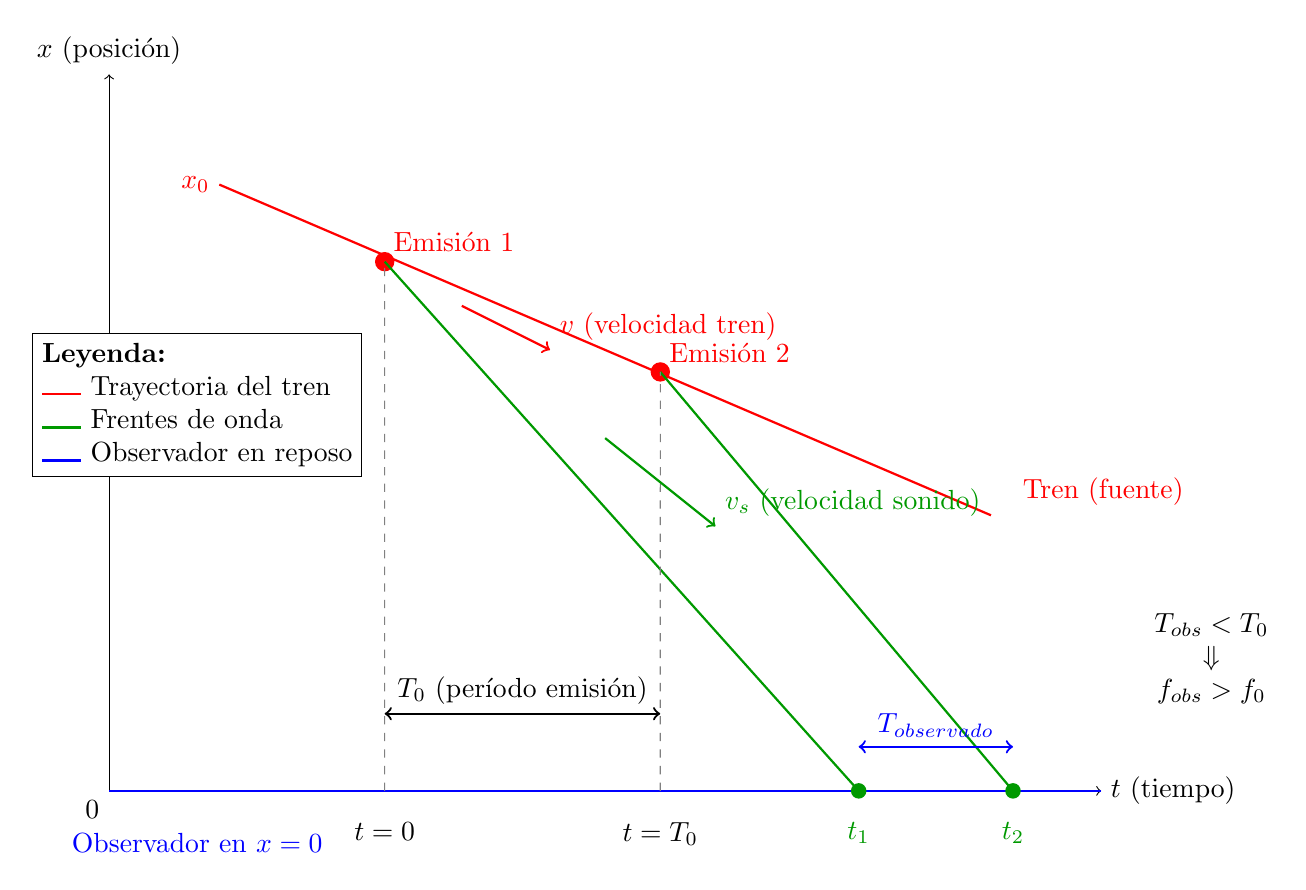
\begin{tikzpicture}[scale=1.4]
    % Ejes
    \draw[->] (0,0) -- (9,0) node[right] {$t$ (tiempo)};
    \draw[->] (0,0) -- (0,6.5) node[above] {$x$ (posición)};
    
    % Etiquetas de los ejes
    \node[below left] at (0,0) {$0$};
    
    % Posición del observador
    \draw[thick, blue] (0,0) -- (9,0);
    \node[below, blue] at (0.8,-0.3) {Observador en $x = 0$};
    
    % Trayectoria del tren (fuente móvil)
    \draw[thick, red] (1,5.5) -- (8,2.5);
    \node[red, above right] at (8.2,2.5) {Tren (fuente)};
    \node[red, left] at (1,5.5) {$x_0$};
    
    % Puntos de emisión
    \coordinate (E1) at (2.5,4.8);
    \coordinate (E2) at (5,3.8);
    \fill[red] (E1) circle (2.5pt);
    \fill[red] (E2) circle (2.5pt);
    \node[red, above, xshift=25pt] at (E1) {Emisión 1};
    \node[red, above, xshift=25pt] at (E2) {Emisión 2};
    
    % Frentes de onda (líneas con pendiente negativa = velocidad del sonido)
    \draw[green!60!black, thick] (E1) -- (6.8,0);
    \draw[green!60!black, thick] (E2) -- (8.2,0);
    
    % Puntos de llegada
    \fill[green!60!black] (6.8,0) circle (2pt);
    \fill[green!60!black] (8.2,0) circle (2pt);
    \node[green!60!black, below] at (6.8,-0.2) {$t_1$};
    \node[green!60!black, below] at (8.2,-0.2) {$t_2$};
    
    % Etiquetas de tiempo de emisión
    \draw[dashed, gray] (2.5,0) -- (E1);
    \draw[dashed, gray] (5,0) -- (E2);
    \node[below] at (2.5,-0.2) {$t = 0$};
    \node[below] at (5,-0.2) {$t = T_0$};
    
    % Período observado
    \draw[<->, blue, thick] (6.8,0.4) -- (8.2,0.4);
    \node[blue, above] at (7.5,0.4) {$T_{observado}$};
    
    % Período de emisión
    \draw[<->, black, thick] (2.5,0.7) -- (5,0.7);
    \node[black, above] at (3.75,0.7) {$T_0$ (período emisión)};
    
    % Velocidades (separadas para evitar superposición)
    \draw[red, ->, thick] (3.2,4.4) -- (4,4);
    \node[red, above right] at (4,4) {$v$ (velocidad tren)};
    
    \draw[green!60!black, ->, thick] (4.5,3.2) -- (5.5,2.4);
    \node[green!60!black, above right] at (5.5,2.4) {$v_s$ (velocidad sonido)};
    
    % Comparación de períodos
    \node[align=center] at (10,1.2) {$T_{obs} < T_0$ \\ $\Downarrow$ \\ $f_{obs} > f_0$};
    
    % Leyenda (reubicada)
    \node[align=left, draw, fill=white] at (0.8,3.5) {
        \textbf{Leyenda:} \\
        \textcolor{red}{\rule{0.5cm}{1pt}} Trayectoria del tren \\
        \textcolor{green!60!black}{\rule{0.5cm}{1pt}} Frentes de onda \\
        \textcolor{blue}{\rule{0.5cm}{1pt}} Observador en reposo
    };
\end{tikzpicture}
\caption{Diagrama de trayectorias $x$-$t$ para el efecto Doppler. El tren (fuente móvil en rojo) emite dos frentes de onda consecutivos separados por un período $T_0$. Como el tren se acerca al observador, el segundo frente se emite desde una posición más cercana, resultando en un período observado $T_{obs} < T_0$, y por tanto una frecuencia mayor.}
\end{figure}

\textbf{Análisis del diagrama:}
\begin{itemize}
    \item La línea roja muestra la trayectoria del tren moviéndose hacia el observador con velocidad $v$
    \item Las líneas verdes representan los frentes de onda propagándose hacia el observador con velocidad $v_s$
    \item El tiempo entre emisiones es $T_0$, pero el tiempo entre llegadas al observador es menor: $T_{obs} = T_0\left(\frac{v_s - v}{v_s}\right)$
    \item Como $T_{obs} < T_0$, la frecuencia observada $f_{obs} = 1/T_{obs}$ es mayor que la emitida $f_0 = 1/T_0$
\end{itemize}

\end{solution}
%--------------------------
\end{questions}
\end{document}